\documentclass{beamer}

\mode<presentation>
{
   \usetheme{EEng}
%   \usetheme{Warsaw}
  \setbeamercovered{transparent}
  \setbeamercolor{background canvas}{bg=black!0}
}

\usepackage{enumerate}
\usepackage{array}
\usepackage{graphics}
\usepackage{ucs}
\usepackage[utf8x]{inputenc}
\usepackage[english]{babel}
\usepackage{amsmath, amsthm, amssymb}
\usepackage{amsmath}
\usepackage{amsfonts}
\usepackage{xcolor}
\usepackage{pgf}
\usepackage{hyperref}
\usepackage{url}
\usepackage{multicol}   % add-on
\usepackage{boxedminipage} 
\usepackage{indentfirst}   % add-on
\usepackage{float}
\usepackage[all]{xypic}
\usepackage{listings}
\usepackage{verbatim}
\usepackage{boxedminipage}

% % % inicio do listings e ref
\definecolor{darkblue}{rgb}{0,0,0.6}
\definecolor{gray_ulisses}{gray}{0.55}
\definecolor{castanho_ulisses}{rgb}{0.71,0.33,0.14}
\definecolor{preto_ulisses}{rgb}{0.41,0.20,0.04}
\definecolor{green_ulises}{rgb}{0.2,0.75,0}

\hypersetup{
    a4paper,
    pdftex,
    bookmarks,
    colorlinks,
    citecolor=darkblue,
    linkcolor=darkblue,
    urlcolor=darkblue,
    filecolor=darkblue
}

\lstdefinelanguage{perl_u} {
       basicstyle=\ttfamily\tiny,
       showstringspaces=false,
       breaklines=true,
       numbers=left,
       numberstyle=\tiny,
       numberblanklines=true,
       showspaces=false,
       showtabs=false
}
% % % fim do listings e ref

\title{GD::Graph - Graph Plotting Module}
\author{José Pedro Silva \and
Pedro Faria \and
Ulisses Costa
}

\date{\today}
\institute{Engenharia de Linguagens\\
Projecto integrado
}

\AtBeginSubsection[] {
  \begin{frame}<beamer>
    \frametitle{Index}
    \scriptsize{\tableofcontents[currentsection,currentsubsection]}
  \end{frame}
}

\AtBeginSection[] {
  \begin{frame}<beamer>
    \frametitle{Index}
    \scriptsize{\tableofcontents[currentsection]}
  \end{frame}
}
\begin{document}
\begin{frame}
   \titlepage
\end{frame}

\begin{frame} \frametitle{Description}
GD::Graph is a perl5 module to create charts using the GD module. The following classes for graphs with axes are defined:
\begin{description}
\item[GD::Graph::lines] Create a line chart.
\item[GD::Graph::bars] Create a bar chart with vertical or horizontal bars.
\item[GD::Graph::linespoints] Combination of lines and points.
\item[GD::Graph::area] Create a graph, representing the data as areas under a line.
\item[GD::Graph::pie] Create a pie chart.
\end{description}
\end{frame}


\begin{frame}[fragile] \frametitle{Overwrite bars - Output}
\begin{figure}[htbp]
\begin{center}
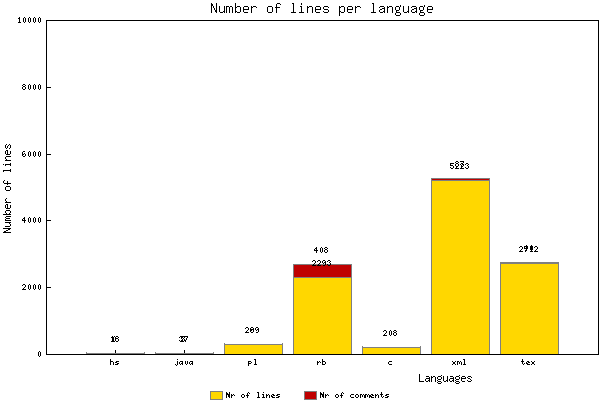
\includegraphics[width=0.9\textwidth]{image/image_LinesPerLanguage.png}
\end{center}
\end{figure}
\end{frame}
\section*{Perguntas}
\begin{frame} \frametitle{Perguntas}
\begin{center}\huge{?}\end{center}
\end{frame}

\end{document}

